%% LyX 2.0.2 created this file.  For more info, see http://www.lyx.org/.
%% Do not edit unless you really know what you are doing.
\documentclass[a4paper,spanish]{article}
\usepackage[latin9]{inputenc}
\pagestyle{empty}
\usepackage{float}
\usepackage{graphicx}

\makeatletter

%%%%%%%%%%%%%%%%%%%%%%%%%%%%%% LyX specific LaTeX commands.
\special{papersize=\the\paperwidth,\the\paperheight}


%%%%%%%%%%%%%%%%%%%%%%%%%%%%%% User specified LaTeX commands.
\pagestyle{empty}
\topmargin=-3.5cm
\oddsidemargin=0cm
\textwidth=16.5cm
\textheight=27.6cm

\makeatother

\usepackage{babel}
\addto\shorthandsspanish{\spanishdeactivate{~<>}}

\begin{document}

\title{\textbf{Implementaci�n de una transformaci�n asociada a un homeomorfismo
entre una regi�n plana simplemente conexa y el disco unitario abierto}\\
 Geometr�a}


\author{Antonio S�ngari, Cristina Eg�ez \\
 %EndAName
Departamento de Matem�tica, Facultad de Ciencias Exactas. \\
 Universidad Nacional de Salta}

\maketitle
Construimos una transformaci�n biyectiva conforme que convierte regiones
$\Omega$ simplemente convexas del plano (distintas del mismo plano)
en el c�rculo unitario abierto $U$, y rec�procamente. En este trabajo
consideramos dominios incluidos en el c�rculo unitario que contienen
el origen y cuya frontera corta solamente una vez los rayos desde
el origen. Para ello usamos el esquema de la demostraci�n del Teorema
de Riemann para transformaciones conformes, realizada por Koebe, que
consiste en la construcci�n iterativa de regiones $\Omega_{1},$$\Omega_{2},\dots$,
a partir de la regi�n $\Omega_{0}=\Omega\subset U$, generadas por
una sucesi�n de funciones $f_{1},f_{2},\dots$, de modo que $f_{i}\left(\Omega_{i-1}\right)=\Omega_{i}$,
y $f_{n}\circ f_{n-1}\circ\cdots\circ f_{1}$ converja a una transformaci�n
conforme $f$ de $\Omega$ sobre $U$. A su vez cada una de las funciones
$f_{i}$ es la composici�n de dos transformaciones bilineales y una
ra�z cuadrada. La demostraci�n este teorema hace uso del hecho que
toda funci�n anal�tica que no se anula en $\Omega$ admite una funci�n
ra�z cuadrada tambi�n an�litica en $\Omega$.

Planteamos una rotaci�n al semiplano de la derecha que nos permite
aplicar luego una ra�z cuadrada anal�tica, y lograr as� un homeomorfismo
entre cualquier regi�n propia del plano, simplemente conexa, y el
disco unitario abierto, como observamos en la figura 1 para dominios
convexos y en la figura 2 para dominios c�ncavos.

\begin{figure}[H]
\begin{centering}
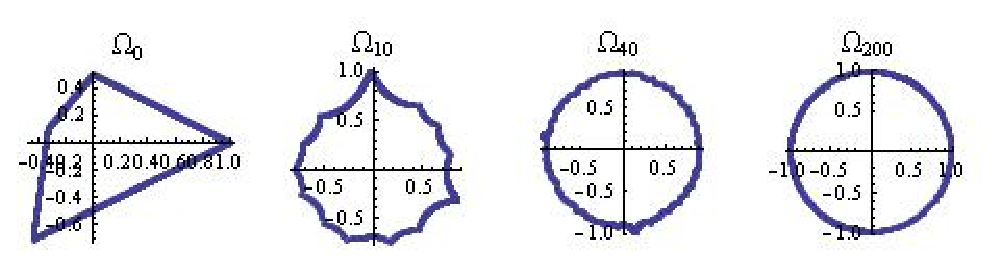
\includegraphics[width=8cm]{convexo}
\par\end{centering}

\begin{centering}
\caption{Dominio Convexo}

\par\end{centering}

\end{figure}


\begin{figure}[H]
\begin{centering}
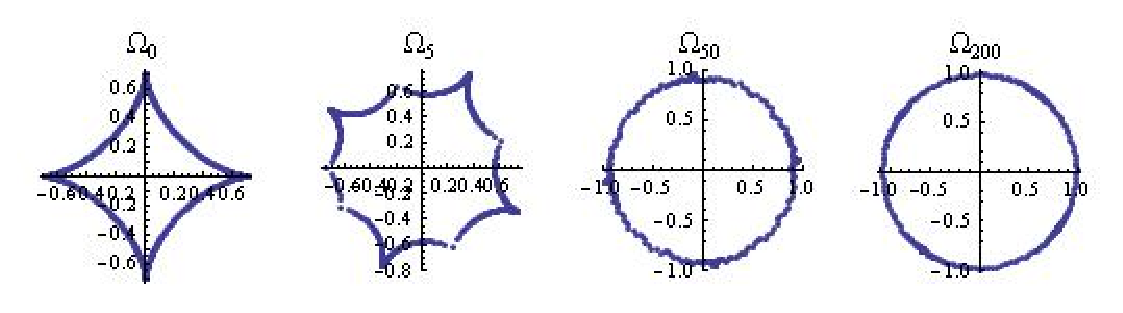
\includegraphics[width=8cm]{concavo1}
\par\end{centering}

\caption{Dominio C�ncavo}


\end{figure}


Elaboramos un paquete inform�tico que construye cada una de las $f_{i}$,
las aplica a la frontera de $\Omega_{i-1}$ y obtiene la frontera
de $\Omega_{i}$. Una vez concluida esta tarea, usando la transformaci�n
inversa, que tambi�n ser� conforme, podemos conseguir una transformaci�n
de $U$ sobre $\Omega$.
\begin{thebibliography}{1}
\bibitem{1} EG�EZ C., S�NGARI A., Aplicaci�n del algoritmo de Koebe
a regiones simplemente conexas, Comunicaciones Cient�ficas. UMA 2010.

\bibitem{2} HILBERT D. and COHN-VOSEN S., Geometry and the Imagination,
Chelsea Publishing Company New York, 1990.

\bibitem{3} NEVANLINNA R., PAATERO V, Introduction to complex analysis.
Addison Wesley Publishing Company, 1969.

\bibitem{4} RUDIN W., Real and Complex Analysis, McGraw-Hill, 1992. \end{thebibliography}

\end{document}
